\documentclass[mathNotesPreamble]{subfiles}
\begin{document}
% \relscale{1.4}
\section{5.2: Definite Integrals}
In section 5.1, we assumed $f$ was nonnegative on the interval $\sbrkt{a,b}$. 

\noindent
When $f(x)\leq 0$ on the interval $\sbrkt{a,b}$, then the area between $f(x)$ and the $x$-axis is negative.
\vspace*{\stretch{1}}
\begin{ex*}
  Consider the function $x^3-1$ on $\sbrkt{-2,0}$. Using Riemann sums, we can approximate the area between the curve and the $x$-axis:
\end{ex*}
\vspace*{15pt}

\hspace*{\stretch{1}}
\begin{tikzpicture}[scale=0.825, declare function={
  f(\x)=\x^3-1; a=-2; b=0; n=4; del=(b-a)/n;
  }]
  \begin{groupplot}[
    group style={group size=3 by 1, horizontal sep=0.5cm},
    axis lines=center,
    axis line style={->},
    xmin=-2.5, xmax=2.5,
    ticklabel style={font=\footnotesize,inner sep=0.5pt,fill=white,opacity=1.0, text opacity=1},
    every axis plot/.append style={line width=0.95pt, color=blue, samples=100}
    ]
    \nextgroupplot 
      \pgfplotsinvokeforeach{a,a+del,...,b-del}{
        \draw[left color=red!95, right color=red!40, line width=0.0pt] 
        (axis cs: #1, 0) rectangle (#1+del, {f(del*0.0+#1)});}
      \addplot[-] expression[domain=-2.015:1.75]{f(x)};
    \nextgroupplot 
      \pgfplotsinvokeforeach{a,a+del,...,b-del}{
        \draw[left color=red!95, right color=red!40, line width=0.0pt] 
        (axis cs: #1, 0) rectangle (#1+del, {f(del*0.5+#1)});}
      \addplot[-] expression[domain=-2.015:1.75]{f(x)};
    \nextgroupplot 
      \pgfplotsinvokeforeach{a,a+del,...,b-del}{
        \draw[left color=red!95, right color=red!40, line width=0.0pt] 
        (axis cs: #1, 0) rectangle (#1+del, {f(del*1.0+#1)});}
      \addplot[-] expression[domain=-2.015:1.75]{f(x)};
  \end{groupplot}
\end{tikzpicture}
\hspace*{\stretch{1}}
\begin{center}
  \parbox{0.8\linewidth}{
  \begin{align*}
    L_4&= f(-2)\frac{1}{2}+f(-1.5)\frac{1}{2}+f(-1)\frac{1}{2}+f(-0.5)\frac{1}{2}&
      &=-8.25\\[\baselineskip]
    M_4&= f(-1.75)\frac{1}{2}+f(-1.25)\frac{1}{2}+f(-0.75)\frac{1}{2}+f(-0.25)\frac{1}{2}&
      &=-5.875\\[\baselineskip]
    R_4&= f(-1.5)\frac{1}{2}+f(-1)\frac{1}{2}+f(-0.5)\frac{1}{2}+f(0)\frac{1}{2}&
      &=-4.25
  \end{align*}}
\end{center}
Actual area: $\boxed{-6}$
\vspace*{\stretch{1}}
\pagebreak
\begin{defn*}[Net Area]
  Consider the region $R$ bounded by the graph of a continuous function $f$ and the $x$-axis between $x=a$ and $x=b$. The \textbf{net area} of $R$ is the sum of the areas of the parts of $R$ that lie above the $x$-axis \textit{minus} the sum of the areas of the parts of $R$ that lie below the $x$-axis on $\sbrkt{a,b}$.
\end{defn*}
\begin{ex*}
  If $f(x)=x^2-2x,\ 0\leq x\leq 3$, evaluate the Riemann sum with $n=6$, taking the sample points to be right endpoints. 

\vspace*{\stretch{1}}
  \begin{tikzpicture}
    \begin{axis}[
      %grid=both,
      %grid style={line width=0.35pt, draw=gray!75},
      axis lines=center,
      axis line style={-},
      xmin=-0.5, xmax=4,
      ymin=-1, ymax=4,
      xtick={0,1,...,3},
      ymajorticks=false,
      ticklabel style={font=\footnotesize,inner sep=1pt,fill=white,opacity=1.0, text opacity=1},
      every axis plot/.append style={line width=0.95pt, color=blue, samples=100}
      ]
    \end{axis}
  \end{tikzpicture}
\end{ex*}

\begin{ex*}
  Find the Riemann sum for $f(x)=\sin(x),\ 0\leq x\leq \frac{3\pi}{2}$, with six terms, taking the sample points to be right endpoints.

\vspace*{\stretch{1}}
  \begin{tikzpicture}
    \begin{axis}[
      %grid=both,
      %grid style={line width=0.35pt, draw=gray!75},
      axis lines=center,
      axis line style={-},
      xmin=-0.6, xmax=4.75,
      ymin=-1, ymax=1,
      xtick={0,1.570796327,...,5},
      xticklabels = {,$\frac{\pi}{2}$, $\pi$, $\frac{3\pi}{2}$},
      ymajorticks=false,
      minor x tick num = 1,
      ticklabel style={font=\footnotesize,inner sep=1pt,fill=white,opacity=1.0, text opacity=1},
      every axis plot/.append style={line width=0.95pt, color=blue, samples=100}
      ]
    \end{axis}
  \end{tikzpicture}
\end{ex*}
\pagebreak

\begin{defn*}[Definite Integral]
  A function $f$ defined on $\sbrkt{a,b}$ is \textbf{integrable} on $\sbrkt{a,b}$ if $\ds\lim_{n\to \infty} \sum\kto^n f(x_k^*)\Delta x_k$ exists and is unique over all partitions of $\sbrkt{a,b}$ and all choices of $x_k^*$ on a partition. This limit is the \textbf{definite integral of $f$ from $a$ to $b$}, which we write
  \[\int_a^b f(x)\,dx=\lim_{n\to \infty}\sum\kto^n f(x_k^*)\Delta x_k\]
\end{defn*}

\begin{center}
  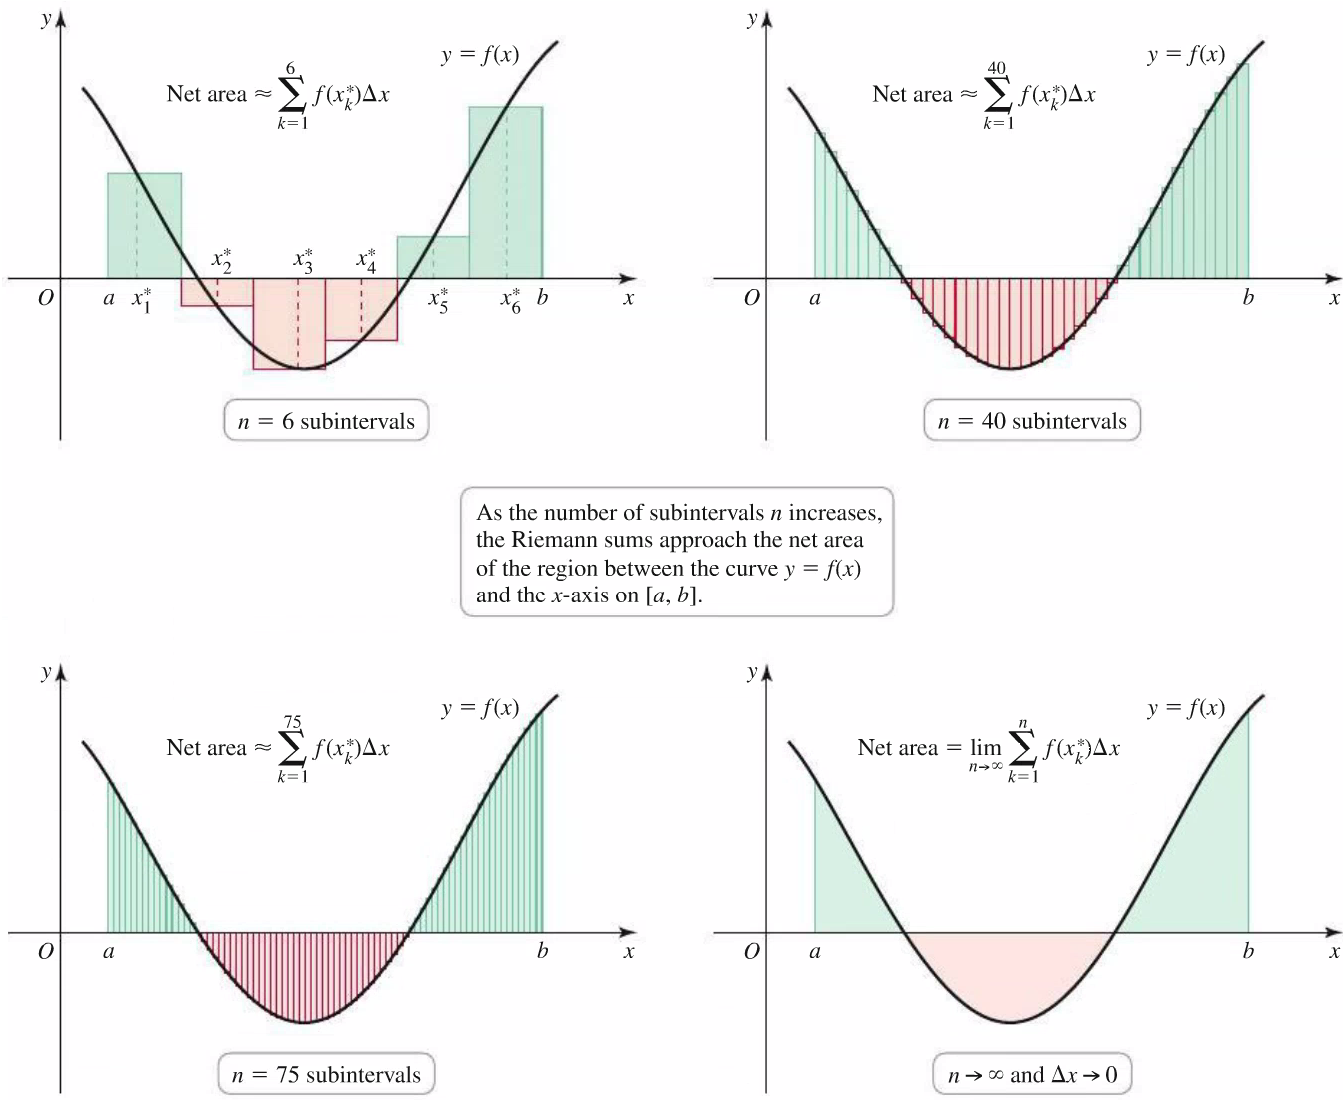
\includegraphics[width=0.85\linewidth]{images/briggs_05_02/fig5_20.png}
\end{center}
\pagebreak
\begin{ex*}~

  \begin{tasks}[after-item-skip=\stretch{1}](1)
    \task 
      For the function $f(x)=3x+2x^2$, find a formula for the upper sum obtained by dividing the interval $\sbrkt{0,1}$ into $n$ equal subintervals.
    \task 
      Take the limit of the sum as $n\to\infty$ to calculate the area under $f(x)=3x+2x^2$ over $\sbrkt{0,1}$.
  \end{tasks}
\end{ex*}
\vspace*{\stretch{0.25}}
\pagebreak

\begin{ex*}
  Use the limit of the Riemann sum notation to evaluate $\ds\int_0^2 (2-x^2)\,dx$.
\end{ex*}
\vspace*{\stretch{1}}
\begin{ex*}
  Use the definition of the definite integral to evaluate $\ds\int_1^4 \parens{x^2-1}\,dx$.
\end{ex*}
\vspace*{\stretch{1}}
\pagebreak

\begin{ex*}
  Use the definition of the definite integral to evaluate $\ds\int_1^4 \parens{x^2-4x+2}\,dx$.
\end{ex*}
\vspace*{\stretch{1}}

\begin{ex*}
  Use the definition of the definite integral to evaluate $\ds\int_0^2 4x^3\,dx$.
\end{ex*}
\vspace*{\stretch{1}}
\pagebreak

\begin{ex*}
  Use a sketch and geometry to evaluate the following integral
  
  $\ds\int_1^{10} g(x)\,dx$, where $g(x)=
  \begin{cases}
    4x,& \textnormal{if } 0\leq x\leq 2\\
    -8x+16,& \textnormal{if } 2< x\leq 3\\
    -8,& \textnormal{if } x>3
  \end{cases}$
\end{ex*}
\begin{tikzpicture}
  \begin{axis}[
    axis lines=center,
    axis line style={-},
    xmin=-0.25, xmax=5,
    ymin=-8.5, ymax=8.5,
    xtick={1,2,...,4},
    ytick={-8,8},
    xticklabels = {,,,},
    width=0.5\linewidth,
    height=2.25in,
    ticklabel style={font=\footnotesize,inner sep=0.5pt,fill=white,opacity=1.0, text opacity=1},
    every axis plot/.append style={line width=0.95pt, color=blue, samples=100}
    ]
  \end{axis}
\end{tikzpicture}

\begin{ex*}
  Use the following figure to evaluate the integrals below:
  \begin{center}
    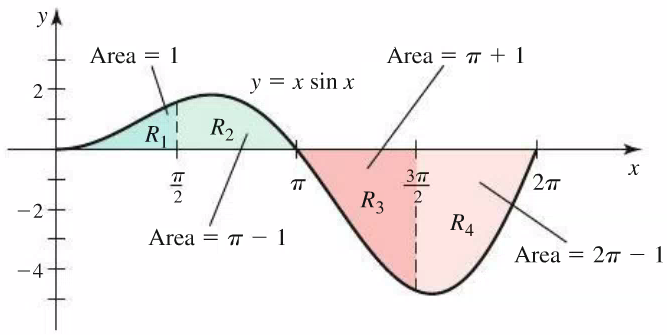
\includegraphics[width=0.4\linewidth]{images/briggs_05_02/q47_50.png}
  \end{center}
\end{ex*}

\begin{tasks}[after-item-skip=\stretch{1}](2)
  \task $\ds\int_{0}^{\pi} x\sin(x)\,dx$
  \task $\ds\int_{0}^{\sfrac{3\pi}{2}} x\sin(x)\,dx$
  \task $\ds\int_{0}^{2\pi} x\sin(x)\,dx$
  \task $\ds\int_{\sfrac{\pi}{2}}^{2\pi} x\sin(x)\,dx$
\end{tasks}
\vspace*{\stretch{1}}
\pagebreak

\begin{ex*}
  Graph the following integrands and compute the areas to evaluate the integrals.
\end{ex*}
\begin{tasks}[after-item-skip=\stretch{1}](2)
  \task $\ds\int_{\sfrac{1}{2}}^{\sfrac{3}{2}} \parens{-2x+4}\,dx$
  \task $\ds\int_{-2}^{4} \parens{\frac{x}{2}+3}\,dx$
  \task $\ds\int_{0}^{3} \parens{\frac{1}{2}x-1}\,dx$
  \task $\ds\int_{-1}^{3} \parens{3-2x}\,dx$
  \task $\ds\int_{-4}^{0} \sqrt{16-x^2}\,dx$
  \task $\ds\int_{-1}^{1} \parens{1+\sqrt{1-x^2}}\,dx$
  \task $\ds\int_{-2}^{1} \abs{x}\,dx$
  \task $\ds\int_{-1}^{1} \parens{2-\abs{x}}\,dx$
\end{tasks}
\vspace*{\stretch{1}}

\pagebreak

\begin{thmBox*}[Properties of definite integrals]
  Let $f$ and $g$ be integrable functions on an interval that contains $a$, $b$, and $p$.
  
  \begin{enumerate}
    \item $\ds\int_a^a f(x)\,dx=0$
    \item $\ds\int_a^b f(x)\,dx=-\int_b^a f(x)\,dx$
    \item $\ds\int_a^b \parens{f(x)\pm g(x)}\,dx=\int_a^b f(x)\,dx\pm \int_a^b g(x)\,dx$
    \item $\ds\int_a^b c\,\!f(x)\,dx=c\!\int_a^b f(x)\,dx$, for any constant $c$
    \item $\ds\int_a^b f(x)\,dx=\int_a^p f(x)\,dx+\int_p^b f(x)\,dx$
    \item The function $\abs{f}$ is integrable on $\sbrkt{a,b}$ and $\int_a^b\abs{f(x)}\,dx$ is the sum of the areas of the regions bounded by the graph of $f$ and the $x$-axis on $\sbrkt{a,b}$.
    \vspace*{-0.5\baselineskip}
  \end{enumerate}
\end{thmBox*}

\begin{center}
  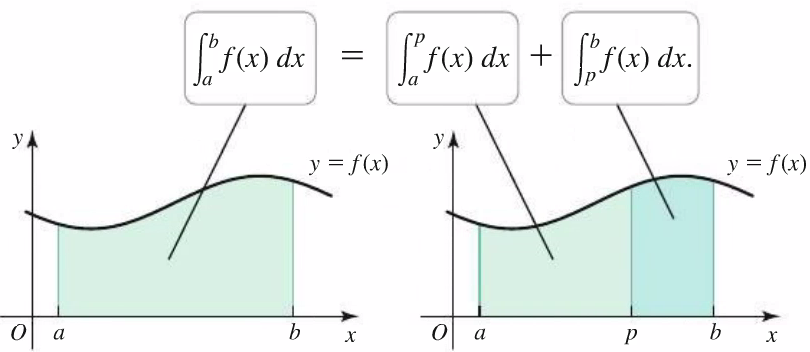
\includegraphics[width=0.475\linewidth]{images/briggs_05_02/fig5_29.png}\\[0.65\baselineskip]
  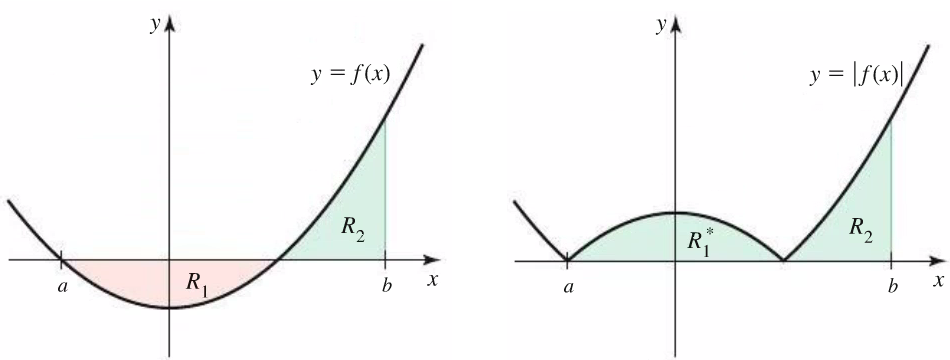
\includegraphics[width=0.475\linewidth]{images/briggs_05_02/fig5_31.png}
\end{center}
\pagebreak
\begin{ex*}
  Suppose that $\ds\int_{-3}^{0} g(t)\,dt=\sqrt 2$. Evaluate the following:
\end{ex*}
\begin{tasks}[after-item-skip=\stretch{1}](2)
  \task $\ds\int_{-3}^{0} g(u)\,du$
  \task $\ds\int_{0}^{-3} g(t)\,dt$
  \task $\ds\int_{0}^{-3} \sbrkt{-g(x)}\,dx$
  \task $\ds\int_{-3}^{0} \frac{g(r)}{\sqrt 2}\,dr$
\end{tasks}
\vspace*{\stretch{1}}

\begin{ex*}
  Suppose that $\ds\int_0^3 f(z)\,dz=3$ and $\ds\int_0^4 f(z)\,dz=7$. Evaluate the following:
\end{ex*}
\begin{tasks}(2)
  \task $\ds\int_3^4 f(z)\,dz$
  \task $\ds\int_4^3 f(z)\,dz$
\end{tasks}
\vspace*{\stretch{1}}
\pagebreak

\begin{ex*}
  Use the fact that $\ds\int_0^{\sfrac{\pi}{2}} \parens{\cos(\theta)-2\sin(\theta)}\,d\theta=-1$ to evaluate the following
\end{ex*}
\begin{tasks}(2)  
  \task $\ds\int_0^{\sfrac{\pi}{2}} \parens{2\sin(\theta)-\cos(\theta)}\,d\theta$
  \task $\ds\int_{\sfrac{\pi}{2}}^0 \parens{4\cos(\theta)-8\sin(\theta)}\,d\theta$
\end{tasks}
\vspace*{\stretch{1}}

\begin{ex*}
  Suppose that $\ds\int_1^9 f(x)\,dx=-1$, $\ds\int_7^9 f(x)\,dx=5$ and $\ds\int_7^9 h(x)\,dx=4$. Evaluate the following:
\end{ex*}
\begin{tasks}[after-item-skip=\stretch{1}](2)
  \task $\ds\int_1^9 -2f(x)\,dx$
  \task $\ds\int_7^9 \sbrkt{f(x)+h(x)}\,dx$
  \task $\ds\int_7^9 \sbrkt{2f(x)-3h(x)}\,dx$
  \task $\ds\int_9^1 f(x)\,dx$
  \task $\ds\int_1^7 f(x)\,dx$
  \task $\ds\int_7^9 \sbrkt{h(x)-f(x)}\,dx$
\end{tasks}
\vspace*{\stretch{1}}
\pagebreak
\begin{ex*}
  Given $\ds\int_1^3 e^x\,dx=e^3-e$, find $\ds\int_1^3 \parens{2e^x-1}\,dx$
\end{ex*}
\vspace*{\stretch{1}}

\begin{ex*}
  Suppose that $f(x)\geq 0$ on $\sbrkt{0,2}$ and $f(x)\leq 0$ on $\sbrkt{2,5}$ where $\ds\int_0^2 f(x)\,dx=6$ and $\ds\int_2^5 f(x)\,dx=-8$. Evaluate the following:
\end{ex*}
\begin{tasks}[after-item-skip=\stretch{1}](2)
  \task $\ds\int_0^5 f(x)\,dx$
  \task $\ds\int_0^5 \abs{f(x)}\,dx$
  \task $\ds\int_2^5 4\abs{f(x)}\,dx$
  \task $\ds\int_0^5 \parens{f(x)+\abs{f(x)}}\,dx$
\end{tasks}
\vspace*{\stretch{1}}
\pagebreak

\end{document}
